% Preamble
% Global
\documentclass[
    parskip=full,
    a4paper
]{scrartcl}
\usepackage{blindtext}
\usepackage[utf8]{inputenc}
\usepackage{etoolbox}

\usepackage{hyperref}
\hypersetup{
    colorlinks,
    citecolor=black,
    filecolor=black,
    linkcolor=black,
    urlcolor=black
}

% Graphics
\usepackage{pdfpages}
\usepackage{graphicx}
\usepackage{xcolor}
\usepackage[many]{tcolorbox}
\usepackage{etoolbox}

% Lists
\usepackage{enumitem}
\setlist{nosep} % or \setlist{noitemsep} to leave space around whole list

% Layout
\usepackage[margin=1in]{geometry}
\usepackage{setspace}
\usepackage[utf8]{inputenc}
\usepackage[english]{babel}
\setstretch{1.3}
% \setlength{\parindent}{0em}
% \setlength{\parskip}{1em}

% Inline-code
\usepackage[outputdir=./_build]{minted}
\definecolor{dhscodebg}{rgb}{0.01,0.199,0.1}
\setminted{
    breaksymbolleft=,
    fontsize=\scriptsize,
    baselinestretch=1.1,
    % bgcolor=dhscodebg,
    % rulecolor=\color{gray!40},
    % framesep=\fboxsep,
    % frame=single,
    % framesep=10pt
    % framerule=2pt,
    xleftmargin=2.5em,
    linenos,
    breaklines,
    tabsize=4
}
\usemintedstyle{tango}
\BeforeBeginEnvironment{minted}
{\begin{tcolorbox}[
            breakable,
            boxrule=0.2pt,
            colback=gray!40,
            % toprule=1pt,
            % rule=1pt,
            arc=0pt
        ]}\AfterEndEnvironment{minted}{\end{tcolorbox}}

% Bibliography
\usepackage{natbib}
\usepackage{bibentry}
\nobibliography*

% Title
\title{Analysing relational datasets with CouchDB's MapReduce implementation}
\author{Zach Smith}
\date{\today}

% Document
\begin{document}

% Title page
\maketitle
\newpage

%  TOC
\tableofcontents
\newpage

% Content
\section{Introduction}
\subsection{Background}

In response to having to dealing with a huge amount of data on a daily basis, authors at Google (Jeffrey Dean and Sanjay Ghemawat) outlined a programming model that abstracted complications associated with distributed computing such as how to parallelize processing, data distribution, fault tolerance, load balancing and execution time \cite{Dean:2008}. This model, known as \textit{MapReduce}, provides programmers a conceptually-simple interface for specifying dispersed data computations succinctly and hides implementation details. The framework relies on an astoundingly simple programming model described by \cite{Dean:2008} as a computation that takes a set of input \textit{key:value} pairs and produces a set of output \textit{key:value} pairs via the following 3 steps:

\begin{enumerate}
    \item A \textit{mapping} stage in which distributed \textit{key:value} pairs are produced from input data as described by a user-defined \textit{map} function
    \item A \textit{grouping} stage where distributed \textit{key:value} output from the mapping stage is collected to common \textit{keys} - i.e. \textit{key:[value, value, value]} datasets
    \item And a \textit{reduce} stage where \textit{values} per key \textit{key} are processed as described by a user-defined \textit{reduce} function
\end{enumerate}

Due to the distributed and isolated nature of \textit{map} and \textit{reduce} tasks, \textit{MapReduce} as an idea is greatly fault tolerant (fault tolerance is implemented via reexecution), which has in turn resulted in the "New Software Stack" as mentioned by \cite{mining2011} - large scale computing clusters built on commodity (cheap) hardware and software that computes in parallel. The "New Software Stack" represents processing ever-greater amounts of data at ever cheaper rates and has spurred information explosion across all manor of software applications.

With the development of the \textit{Hadoop} framework as an open-source alternative to Google's proprietary file system and MapReduce framework, data computations within a MapReduce context have become mainstream. As \cite{chandar2010} discusses in his MSc thesis "Join Algorithms using Map/Reduce" made available by the University of Edinburgh, many companies now utilize this idea including Yahoo, Facebook, Amazon and many others (The Apache Foundation maintains a list of companies that use the Hadoop framework \cite{hadoopPower:2017}).

With increasing update within a data-analysis context, it is fair to say that many of the algorithms required on a day-to-day basis in common data-querying tasks can be implemented via the MapReduce framework including \textit{relational-algebra} operations such as \textit{selection}, \textit{projection} (selection of a subset of attributes from a tuple), \textit{union}, \textit{intersection}, \textit{difference}, \textit{joins} (non-equi joins cannot be implemented via MapReduce), \textit{grouping} and \textit{aggregation} \cite{mining2011}.

As mentioned by \cite{chandar2010} both \textit{Two-Way} and \textit{Multi-Way} joins can be implemented via the MapReduce framework in general, though this is dependent on specific implementations of MapReduce. \textit{Two-Way} joins can be achieved via MapReduce using \textit{Reduce-Side Join}, \textit{Map-side Join}, and \textit{Broadcast Join} algorithms. As the subject of his thesis, \cite{chandar2010} outlines and measures performance for \textit{Multi-Way} joins using \textit{Map-Side Join}, \textit{Reduce-Side One-Shot Join},\textit{Reduce-Side Cascade Join} algorithms. The author found that \textit{Multi-Way} joins were feasible using MapReduce, and that implementation complications of a dispersed system were hidden (as expected) by the Hadoop framework. In other words, \cite{chandar2010} found that relational operations are feasable within dispersed systems running the MapReduce framework.
% \bibliography{../bibliography/msc_citations}

\subsection{Motivation \& Aim}
Compared to RDMSs such as Sql Server, Oracle, MySQL, and many others, CouchDB offers the advantages of scheme-less data-modeling, an HTTP interface and easy-to-setup clustering. These features make for a variety of use-cases that makes research into using CouchDB worthwhile. And because the software is completely open-source, it is free to use.

The clustering features added when IBM's Cloudant software was merged for the 2.0 release allow CouchDB databases to handle a theoretical unlimited amount of data, with indexes calculated in a truly dispersed way (indexes are calculated partially and in parallel across any number of nodes). Replicated shards also allow for node-failure, meaning that (theoretically) CouchDB allows for unlimited storage on clusters of cheap virtual servers.

CouchDB's native HTTP (RESTful) API combined with JSON storage makes the database 'web'-like, meaning that interactions with the data-layer (from a server) are reminiscent of interacting with web 2.0 applications. This is very easy, and since browser requests are over HTTP(S), it is possible to interact with the database directly with a browser. Combined with CouchDB's handling of file data (attachments), and a couple other features (show functions, list functions, URL rewrites and a vHost engine to name a few) CouchDB can double as a webserver that serves HTML. The CouchDB community has traditionally referred to serving HTML as "CouchApps". These tools allow for designing bespoke database-management tools very quickly and were definitely a CouchDB draw-card for many as seen in this open email exchange \cite{googleCon2017}. This same exchange shows (unfortunately) that the "CouchApp" feature of CouchDB is unlikely to survive future releases due to lack of interest in contributing to this feature.

todo: schemaless json
view index flattens json
\subsection{Related Work}

\section{CouchDB}
% \bibliography{../bibliography/msc_citations}

\subsection{CouchDB's MapReduce implementation}
"CouchDB: The Definitive Guide" summarizes the database as appearing to be "a B-tree manager with an HTTP interface" \cite{couchguide}, due to the nature of how the database handles both its data and its indexes. CouchDB's MapReduce API actually allows for defining indexes rather than queries; a user is given direct access to the raw indexes, unlike other DBMSs such as SQL Server where indexes are kept behind the scenes and used instead to facilitate result fetching.

More accurately, \textit{map} results are stored as B+ indexes within CouchDB and \textit{reduce} results are stored as internal nodes on this B+ tree \ref{appendix:rnewson}. CouchDB's \textit{reduce} implementation is optimized to \textit{rereduce} when processing large numbers of documents dictated by the structure of the B+tree. As mentioned on the original (and no longer maintained) CouchDB Wiki, \textit{map} output is sent the \textit{Reducer} in batches delimited by B+tree boundaries \cite{couchwiki}. Since grouping is done after this step by the \textit{Reducer}, there is no guarantee that all values relating to a specific key (as produced by the \textit{map} function) will be processed by the same \textit{reduce} function. CouchDB user-defined \textit{reduce} functions had to implement a confusing contract instead. A \textit{reduce} function should handle the case when \mintinline{javascript}{rereduce = fals;} and when \mintinline{javascript}{rereduce = true;} - see \ref{couchmapreduce}. It is possible that the same logic can be used for either case, as in the CouchDB built in \mintinline{javascript}{_sum} function, but largely the two cases require separate logic.

Because of the nature of the \textit{reduce} function contract, joins that are possible via algorithms described by \cite{chandar2010} are simply not possible. A SQL query of the form: \textit{R(a,b)} joined with \textit{S(b,c)} joined with \textit{T(c,d)} (where \textit{R}, \textit{S} and \textit{T} are relations and \textit{a}, \textit{b}, \textit{c}, \textit{d} are attributes) and expressed by the code (SQL Server syntax):

\begin{minted}{sql}
SELECT
[R].[a],
[T].[d]
FROM [R]
LEFT JOIN [S] on [S].[b] = [R].[b]
LEFT JOIN [T] ON [T].[c] = [S].[c]
\end{minted}

cannot be achieved without prior processing of all or some of the relations, or in the spirit of CouchDB, via multiple queries. If two or more entities were to be joined on a common field then it is theoretically possible to group these values in the reduce function and retrieve a 'joined' dataset that way, but CouchDB looks for this and warns users that this is NOT an appropriate use of MapReduce. CouchDB's optimization of it's B+tree storage structures means that the database complains when \textit{reduce} function output doesn't shrink compared to the input. There is a configurable setting in CouchDB \mintinline{javascript}{reduce_limit=false} that allows a user to override the default setting, but as mentioned in this project, such a configuration produced no results within a reasonable time frame. As one of the owners of CouchDB mentions, such a function would defeat the purpose of structuring the view results as an index and result in performance in terms of space and time of O(n^2) or worse \ref{appendix:jan_slack}.

Instead it is fair to say that using CouchDB, the full scope of data querying as typically done on RDBMS systems is entirely possible, when such queries are re-imagined to work within the framework of MapReduce. Although other implementations of MapReduce (for example as mentioned by \cite{chandar2010}) do allow for relational operations such as \textit{union} of sets, it is likely that there are more performant ways of analyzing the same data in ways that favor the MapReduce framework (and cannot be achieved using a RDBMS).
\subsection{Queries in CouchDB}

CouchDB uses the concept of "Design" documents that are, like any other CouchDB document, JSON strings. But these documents are treated as interfaces to the server process allow for users to define and execute certain functions. The entire list of functions that users are allowed to define are:

\begin{enumerate}
    \item View Functions
    \item Show Functions
    \item List Functions
    \item Update Functions
    \item Filter Functions
    \item Validate Document Update Functions
\end{enumerate}

For the purpose of this project only \textit{view functions} (The CouchDB MapReduce API), and \textit{list functions} will be discussed. List functions fall under the category of \textit{CouchApps} that as mentioned previously are likely to be excluded from future releases. These functions iterate a view output to an HTTP(S) client, allowing a final phase of transformation - i.e. a data format switch from JSON documents to CSV format. Since \textit{list functions} form part of the HTTP API, these functions effectively allow for "insta-APIs" available to the world - a useful feature and will be discussed later.

\textit{View functions} comprise \textit{Map} and \textit{Reduce} functions. These functions have the form:

\begin{figure}[h]
    \centering
    \begin{minted}{javascript} 

        /**
         * Map function
         * @param  {Object} doc Each document in the database is passed in turn to the function
         * @return {null} Nothing is returned - key:value pairs are emitted (multiple pairs can be emitted per document)
         */
        function(doc) {
            emit(someKey, someValue);
        };

        /**
         * Reduce function
         * @param  {Object[]} [keys] A list of [key, docId] pairs - key as from the map function, and key from the original doc
         * @param  {Object[]} values Output from the map function, or from the reduce function
         * @param  {Boolean} [rereduce] Indicates whether values are output from the map (rereduce = false) or reduce (rereduce = true) function
         * @return {[type]}
         */
        function(keys, values, rereduce) {
            return // ...someValue
        };
    \end{minted}
    \caption[test1]{test2}
    \label{couchmapreduce}
\end{figure}

\subsection{Cluster Setup}
CouchDB is a new animal on the database market, with development started by xxx in xxx primarily as a tool to xxx. The current release, CouchDB 2.1 has a variety of features that may finally make it feasible to replace the way technology has traditionally been used in workplace roles. A summary of CouchDB's key features is:

\begin{enumerate}
    \item Semi-structured data storage allows for easier use by people without prior database experience
    \item An HTTP interface effectively brings database communication out of the stone age and makes interacting with a database on a low level accessible to anyone who can code a line of JavaScript
    \item A MapReduce-based query engine allows for easily creating indexes that can be calculated via distributed computing
    \item And very easy/cheap cluster setup when compared to traditional DBMSs
\end{enumerate}

With these benefits in mind, this project explores the usage of CouchDB as a persistent (but temporary) dispersed data-processing engine for student data in the form of:

\begin{enumerate}
    \item A tool for easily configuring CouchDB clusters with enough nodes to handle the required data volume
    \item An approach for easily designing CouchDB MapReduce indexes, implementing them and running them
\end{enumerate}

CouchDB is open-source software with free binary distributions for a Windows, Max, and Linux environment. With the intent of clustering many server instances, each with it's own instance of the CouchDB software, only Linux is feasible since it is released as free software (GPL license). Combined with affordable, virtual, managed servers such as those offered by Digital Ocean, AWS, Hetzer, Linode to name a few (including several South Africa-based companies), clustered computing is very much within the reach of everyday consumers. Setting up several Ubuntu Xenial/CouchDB 2.1 instances is no more complicated than running a few commands on a Linux terminal. While there is still some technical understanding required in terms of security, it would be fairly straightforward to package 'setup' scripts for non-technical users giving users the potential to utilize CouchDB clusters in their own right.

For the purposes of this MSc, several instances of Hetzner's CX20 virtual cloud servers were used. xxx

A complete list of the commands required for a basic installation of an Ubuntu Xenial server supporting a CouchDB 2.1 installation is as follows:

\begin{minted}{sh}
# Set hostname of server
hostname <hostname>; rm /etc/hostname; touch /etc/hostname; echo <hostname> >> /etc/hostname; chmod 466 /etc/hostname;

## Install basic tooling 
# GCC collection (GNU make and GNU compiler tools)
apt-get update
apt-get install build-essential -y

# Update openssl to 1.0.2l
cd /usr/src
wget https://www.openssl.org/source/openssl-1.0.2l.tar.gz
tar -zxf openssl-1.0.2l.tar.gz
cd openssl-1.0.2l
./config
make
make test
make install
mv /usr/bin/openssl /root/
ln -s /usr/local/ssl/bin/openssl /usr/bin/openssl

# Python
apt-get update
apt-get install python -y

# libcurl
apt-get update
apt-get install libcurl4-openssl-dev -y

# ICU
apt-get update
apt-get install libicu-dev -y

# (Optional - this enables automated installations) preseed debconf to answer CouchDB installation wizard automatically
debconf-set-selections <<< 'couchdb couchdb/bindaddress string 0.0.0.0'
debconf-set-selections <<< 'couchdb couchdb/cookie string monster'
debconf-set-selections <<< 'couchdb couchdb/mode string clustered'
debconf-set-selections <<< 'couchdb couchdb/nodename string couchdb@<hostname>'
debconf-set-selections <<< 'couchdb couchdb/adminpass password <password>'
debconf-set-selections <<< 'couchdb couchdb/adminpass_again password <password>'

# register CouchDB package with the server package manager and install
echo 'deb https://apache.bintray.com/couchdb-deb xenial main' | sudo tee -a /etc/apt/sources.list
curl -L https://couchdb.apache.org/repo/bintray-pubkey.asc | sudo apt-key add -
apt-get update
apt-get install couchdb -y
\end{minted}

And then once those commands have been run to setup all the CouchDB nodes, the CouchDB cluster can be configured using a few commands on any one of the nodes (the coOrdinatingNodeHost):

\begin{minted}{sh}
# Run these two lines to add a node to the CouchDB cluster
curl -X POST -H \"Content-Type: application/json\" http://<username>:<password>@<CoOrdinatingNodeHost>:<port>/_cluster_setup -d '{\"action\": \"enable_cluster\", \"bind_address\":\"CoOrdinatingNodeHost\", \"username\": \"<username>\", \"password\":\"<password>\", \"port\": <port>, \"node_count\": \"<intented node count>\", \"remote_node\": \"<remote hostname>\", \"remote_current_user\": \"<username>\", \"remote_current_password\": \"<password>\" }'
curl -X POST -H \"Content-Type: application/json\" http://<username>:<password>@<CoOrdinatingNodeHost>:<port>/_cluster_setup -d '{\"action\": \"add_node\", \"host\":\"<remote hostname>\", \"port\": \"<port>\", \"username\": \"<username>\", \"password\":\"<password>\"}'

# Finalize the cluster setup
curl -X POST -H \"Content-Type: application/json\" http://<username>:<password>@<CoOrdinatingNodeHost>:<port>/_cluster_setup -d '{\"action\": \"finish_cluster\"}'
\end{minted}

xxx add sources for commands

In other words, installing CouchDB on Ubuntu 16.04 is not very difficult. Due to the testing requirements of this project, a Ruby script was created to automate this process and can be found at \url{https://github.com/zachsa/rcluster}. For a user, the process of installing a clustered CouchDB database now becomes a matter of adjusting a configuration object, which could be a file called 'config.json' and look like this:

\begin{minted}{json}
{
    "PrivateKey": "</path/to/id_rsa>",
    "knownHostsDir": "</path/to/known_hosts>",
    "Servers": [
        "n1.hostname.com",
        "n2.hostname.com",
        "n3.hostname.com",
    ],
    "User": "root",
    "CouchUser": "admin",
    "CouchPswd": "password",
    "CouchBindPort": 5984,
    "DBs": [{
            "name": "db1",
            "q": 8,
            "n": 3
        },
        {
            "name": "db2",
            "q": 8,
            "n": 3
        }
    ]
}
\end{minted}

And then creating a clustered database from scratch with the following command: \mintinline{ruby}{ruby init.rb}, or perhaps just double clicking on an executable in the same folder as the JSON configuration file. As virtual cloud server providers mature and add functionality, setting up clusters becomes even easier. The simple rCluster script presented in this MSc could very easily be extended to script the actual server registration as well.

For this project registering the CX20 instances required logging into the Hetzer.de website and manually ordering the 6 servers that this project utilizes. But the API available at \url{https://robot.your-server.de/doc/webservice/en.html#preface} allows for automation of the process of ordering and provisioning servers. It would not be difficult to extend the rCluster script to allow for automated server ordering. In which case, the script could easily be adjusted to setup thousands of servers at a time. i.e. CouchDB MapReduce queries could easily be dispersed among thousands of computer nodes, as could massive amounts of data. In terms of usability, and following on from the metaphor of Microsoft Excel, it would be of about equivalent difficulty to use a CouchDB cluster of 10 000 + nodes to process a dataset of several TB as it would be to do a similar analysis of a smaller amount of data on Microsoft Excel.

TODO: couchapp with MapReduce queries

\subsection{The Queries}

CouchDB uses the concept of a controller JSON document in which the server is configured. This document allows the user to write scripts that are executed on the server - including the 'map', 'reduce' and 'list' functions - the three components of querying data in CouchDB clusters that allows for mimicking what would otherwise require a RDBMS. Amongst other things, CouchDB design documents allow for:

\begin{enumerate}
    \item Specifying MapReduce query functions
    \item Specifying List/Show functions
    \item Specifying binary attachments (with referenced content type - i.e. jpeg/html/json/png/etc.etc.)
\end{enumerate}

Because attachments as defined in \_design documents can be retrieved via HTTP and can be of content type text/html, a well-known use-case of CouchDB is that it can be used to serve web content. Such webcontent falls under the category 'couchapps'. these are effectively elaborate \_design documents. Several tools exist to facilitate building couchapps. For this MSc, an open source tool available at xxx was used to allow for writing CouchDB query functions in an offline environment. The sourcecode for the 'couchapp' that is CouchDB query instructions can be found here xxx.

\section{nETL}
\subsection{Overview}
Many software packages exist to facilitate data processing; spreadsheet programs such as Microsoft Excel (or their online competition Google Sheets), databases such as Microsoft Access, MySQL are designed for this time of work.

But these tools fail when looking at scale of storage that Sakai's event data requires either in terms of ability (Microsoft Excel can work with a theoretical maximum of around 1 million lines, Access databases can be maximum 2GB), complexity or cost.

This thesis looks at creating a cost-effective 'analysis-engine' capable of scaling to many times the amount of data that a single machine can hold in a way that is still effective to analyze (distributed computing) and not too mentally taxing to implement.

specifically this project analyzed the viability of a software package called CouchDB, a NoSQL DBMS as a replacement for conventional RDMSs when analyzing data that has conventionally been housed RDBMSs (usually with an Oracle, Microsoft or SAP price tag associated with it).

Coming from a relational database environment there are a plethora of tools avaialable that facilitate transfer of CSV dato to a DBMS. These tools are available at a variety of different levels of extraction depending on a users technical skillset, time constraints and requirements. xxx: list some of these tools.

In a SQL Server environment SSDT (formerly SSIS) is considered the de facto standard for extracting/transforming and loading data between different data sources. xxx: find a graph on the usage of SSDT/SSIS in companies.

In fact it's likely that the availability of of SSDT/SSIS has influenced the uptake of SQL Server in operations that require dealing with large amount of data. It's fair to say that a barrier to using open source software such as CouchDB is the LACK of such software. Bespoke scripts are currently the only viable way of interfacing with CouchDB in a way that is comparable to SQL Server and SSDT. But with high-level languages such as node.js maturing, and the proliferation of small, focused libraries in these languages that abstract much of the unpleasant and gnarly aspects of bespoke scripting (xxx examples), bespoke data-scripting is nowhere near as difficult as it would be within the Microsoft environment (C\# or VB).

In line with the requirement of transferring large amounts of CSV data from a CSV source to CouchDB, and taking into account the comparatively low entry barrier to bespoke data-transformation scripts, a component of this MSc is an exploration of a possible alternative to SSDT for an environment other than Microsoft's SQL Server. This MSc project actually has several requirements that fall within the ETL spectrum that such a framework could easily be adapted to handle in a generic way. The framework has been published as an npm library and is available at ..., with source code available at github somewhere xxx.
\section{Design}

\begin{figure}[h]
    \centering
    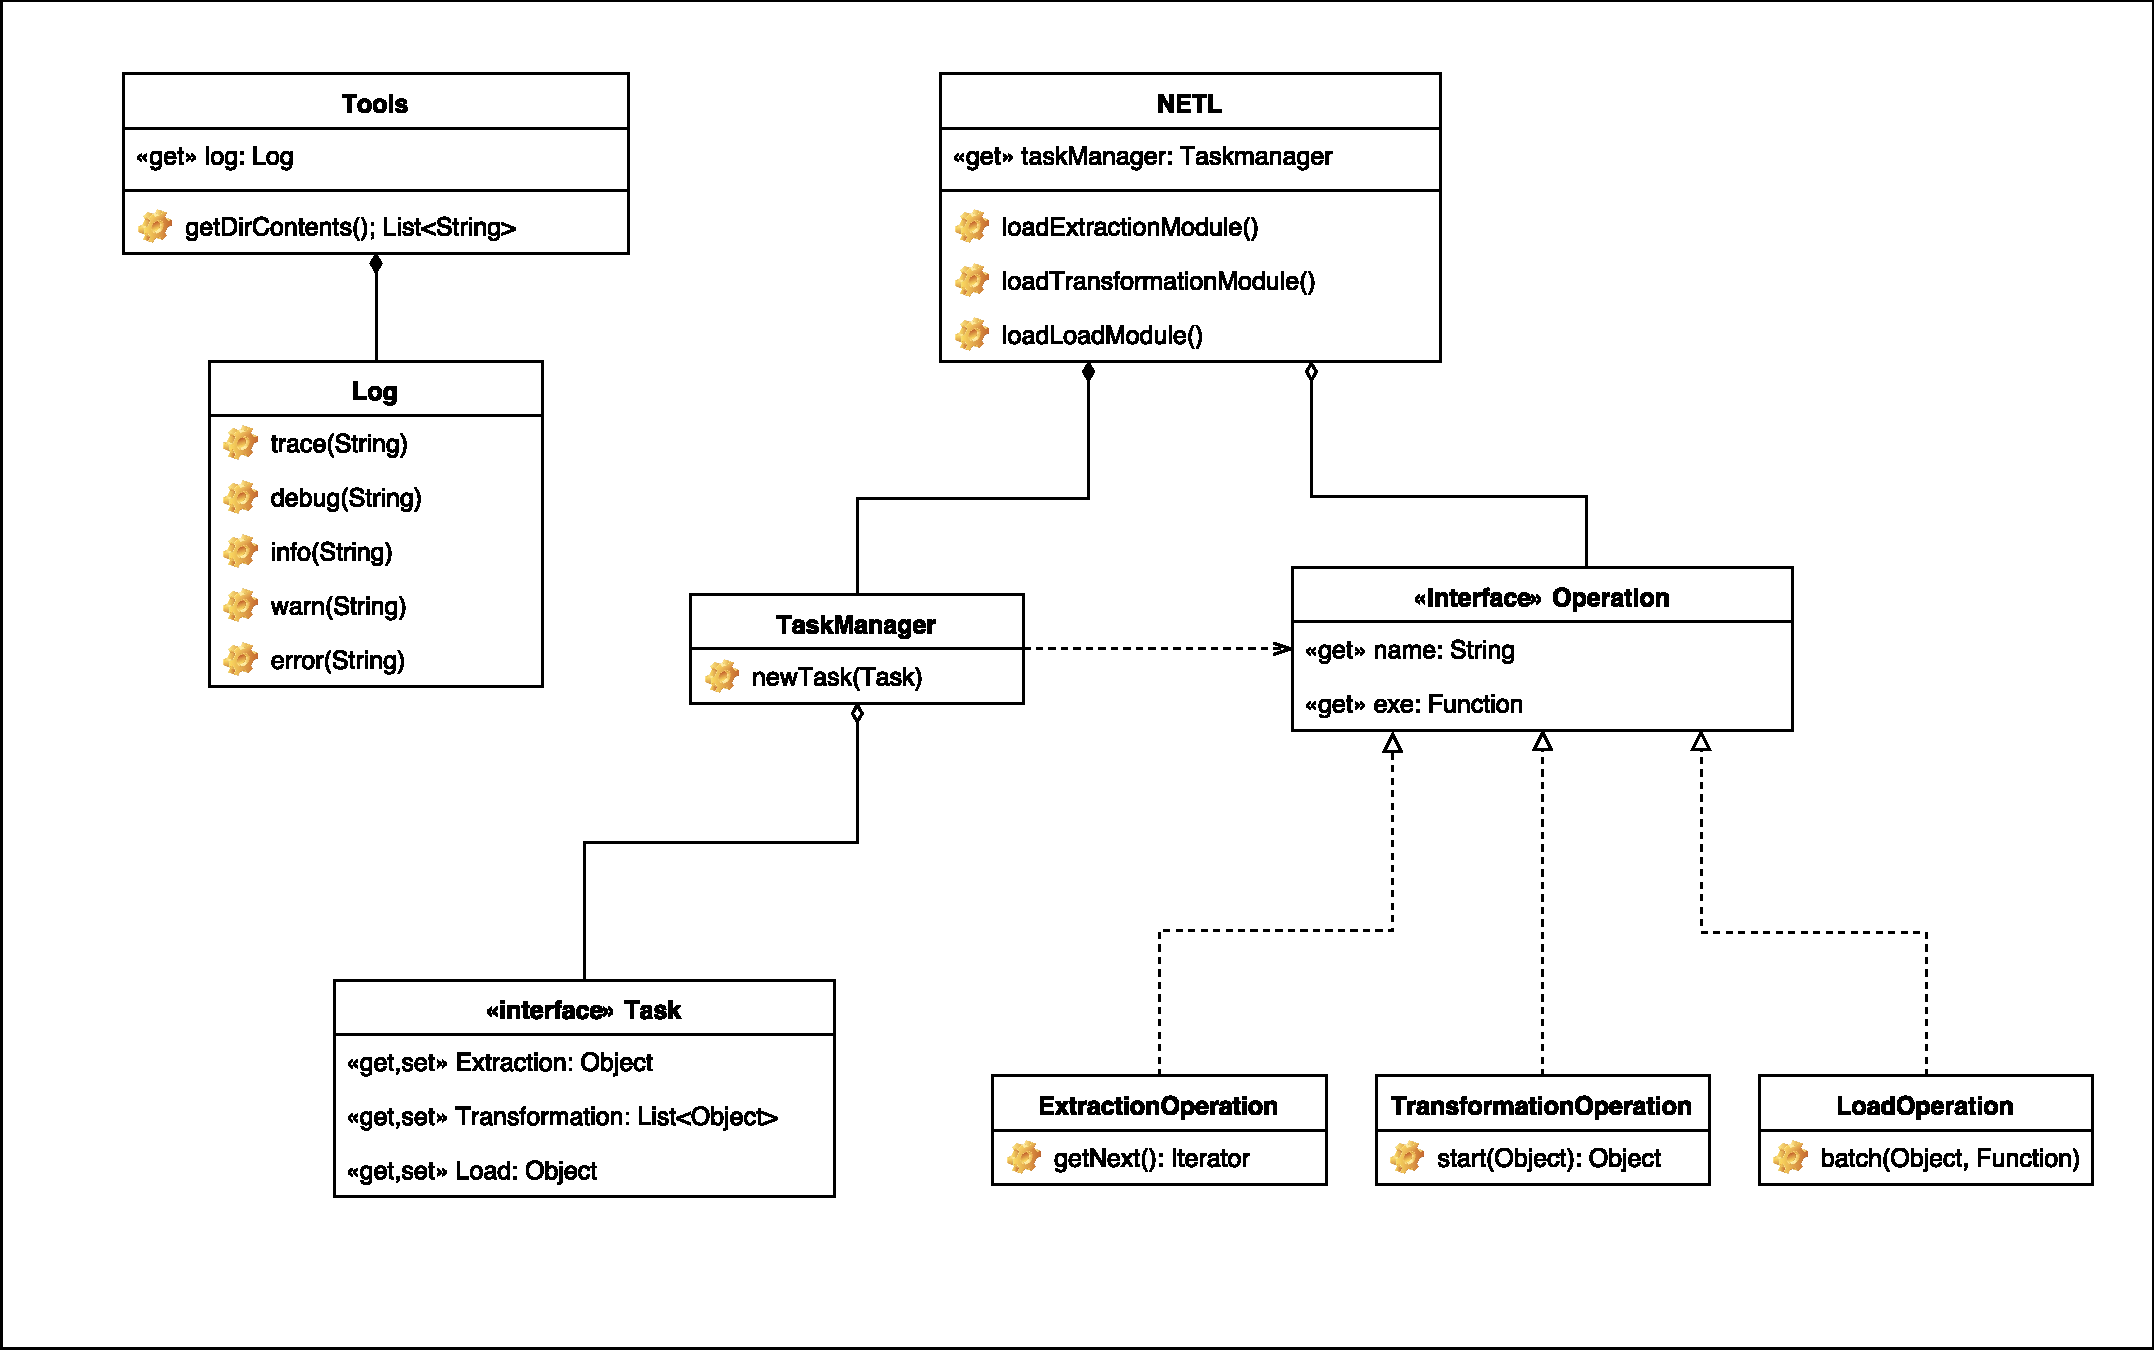
\includegraphics[scale=0.4]{./resources/figures/netlUML}
    \caption[nETL]{nETL}
    \label{nETL}
\end{figure}

Figure \ref{nETL} shows a potential architecture for a configurable component-based ETL tool. The intention of the framework is that it works on the basis of a pipeline of tasks. These tasks can be divided into 3 steps; an extraction step, a transformation step and a loading step. xxx insert something about ETL variations and why I chose the ETL pipeline.

\begin{enumerate}
    \item Extract data from a source specified by a user into memory
    \item Apply any number of transformations to the data in memory
    \item Load the data from memory into a destination specified by a user
\end{enumerate}

The framework itself is quite lightweight and comprises just the NETL, TaskManager and general purpose 'Tools' classes. For the purposes of this thesis, the framework as described by Figure \ref{nETL} has been prototyped in node.js with the source code available at xxx (there is also an npm package available at xxx). JavaScript is a suitable language to prototype this application for a number of reasons:

\begin{enumerate}
    \item It has a very succinct API making it fast to write code in (i.e. it is a highly abstracted language similarly to Ruby or Python)
    \item But unlike Ruby or Python (and other high level languages), it is opinionated in that it handles IO asynchronously by default
    \item The JavaScript implementation of object-orientation allows for easy runtime manipulation of the object model
    \item Another reason for choosing JavaScript is that it is very much in line with the spirit of CouchDB and the web in general
\end{enumerate}

nETL is primarily a task-managing application, and as such, the TaskManager class is effectively the core of the application. It is intended that it can be instantiated as an instance (i.e. there can be many TaskManager instances hosted within a single running application). In JavaScript this is best implemented via a constructor:

\begin{minted}{javascript}
/* File taskmanager.js */
function TaskManager(extractions, transformations, loads) {
    this.tasks = {};

    // Hold references to extractions/transformation/loads of the main application process
    this.extractions = extractions;
    this.transformations = transformations;
    this.loads = loads;
};

TaskManager.prototype.newTask = function(task) {
    // Add task to this.tasks and execute the task
};

module.exports = TaskManager;
\end{minted}

The application itself is intended to be singleton instance of \mintinline{javascript}{class NETL{}}, which provides an IO interface (either a console terminal or otherwise) to TaskManager instances, and modular extraction/transformation and load operations. Singleton's are typically implemented via the modular pattern in JavaScript, which is typically how libraries are delivered to users by package managers and invoked by \mintinline{javascript}{var library = require('library-name')();}. One possible way of implementing the NETL class in JavaScript (i.e the method that is used within this project's code base) is shown here:

\begin{minted}{javascript}
/* File netl.js */
module.exports = function() {
    // Private properties / methods
    const _extractions = {};
    const _transformations = {};
    const _loads = {};        
    const _taskManager = new TaskManager(_extractions, _transformations, _loads);
    function _loadExtractionModule(extractionOperation){};
    function _loadTransformationModule(transformOperation){};
    function _loadLoadModule(loadOperation){};

    // Make process API available
    return {
        taskManager: _taskManager,
        loadExtractionModule: _loadExtractionModule,
        loadTransformationModule: _loadTransformationModule,
        loadLoadModule: _loadLoadModule
    };
};
\end{minted}
\subsection{Implementation}
Since extraction \ensuremath{\rightarrow} transformation \ensuremath{\rightarrow} load pipelines are defined via user-configuration, line data-structures can effectively be replaced by any data structure a user desires. Of course that user needs to make sure that the pipeline component (module) at any point in the pipeline can handle the data structure passed to it.

In any case, once a batch of x lines (or any other kind of data structure) has been obtained, transforming and loading data is pretty easy. Pseudocode to implement the nETL framework task-engine could be written something along the lines of:

\begin{minted}{javascript}
// An IIFE is used effectively as an asynchronous implementation of a while loop
(function doEtlTask(self) {
    var payLoad = [];
    var batch = getBatch.next();

    // Apply transformations to elements of extracted batch
    batch.forEach(function(datum){
        SpecifiedTransformations.forEach(function(t) {
            datum = self.transformations[t.Name].call(t, t).start(datum);
        });
        payLoad.push(datum);
    });

    // Load the batch
    self.load.batch(payLoad, function(status, msg) {
        doEtlTask(self); // Start ETL of next batch
    });

})(/* bind task configuration object to function execution context */);
\end{minted}
\subsection{Usage}

\subsubsection{Extractions}
The framework above has been conceptualized primarily as a means of working with CSV data as exported from the Sukai platform. Specifically, this MSc has the dual requirements of extracting data from an 80GB CSV and snonymising column(s) in this 80GB CSV in a predictable way. To this end, included in the nETL source code used to complete this thesis is a FLATFILE extraction module.

Ethical clearance to use student data, although granted by the University of Cape Town still makes the condition that identities of the students be anonymized. Partly as a way of testing the nETL framework as mentioned above, I offered to provide a 'one-click' installation of the nETL application that provides an anonymizing pipeline for use by Professor Sonia Berman to prepare the student data for this project.

Extracting data from a flatfile is only tricky if it's size is such that the memory footprint of file contents is greater than the memory made available to the process. For an 80GB CSV that is certainly the case. The only feasible means of extracting data from such a file is to utilize the concept of an 'iterator'. Effectively this involves specifying the size of a reading block via two pointers (a 'begin' and 'end' pointer) that then traverse the data structure of the file from start to finish. These pointers maintain a constant width apart and at each incrementation of the iteration retrieve the data between those pointers.

Using an iterator, it is straightforward to process portions of a file at time, so long as only partial retrieval of a file's data can still be understood. Flatfile's work well for this with data structured as any number of 'line' entities that don't need to be read in the context of other marker's that may be found within the file.

Almost all high-level languages provide numerous abstractions for reading flatfile's on a line-by-line basis. For example, in a few different languages file iterators can be generated in the following ways:

\paragraph*{Python}
\begin{minted}{python}
with open('/path/to/file') as file:
   for line in file:
       # Process the line
\end{minted}

\paragraph*{Ruby}
\begin{minted}{ruby}
IO.foreach('/path/to/file') do |line|
  # Process the line
end
\end{minted}

\paragraph*{C\#}
\begin{minted}{csharp}
using (StreamReader streamReader = File.OpenText(/path/to/file))
{
    string line = String.Empty;
    while ((line = streamReader.ReadLine()) != null)
    {
        // Process the line
    }
}
\end{minted}

JavaScript provides a similar API for reading files line-by-line to the languages mentioned above, and a user could write such a simple iterator module provided that the module adhere to the nETL module interface for extractions and implements a \mintinline{javascript}{getNext()} function that effectively allows for pausing such extraction. It's likely that there are numerous ways of achieving this with the standard ECMAScript 5 standard. But partly as a means of exploring more state-of-the art JavaScript features, and partly of a means of demonstrating these new features, the file extraction module as used in this thesis implements EcmaScript 6 generators.

As described by \cite{mozillaGenerators}, JavaScript generators allow for quickly implementing arbitrary iterators, including iterators over generated iterators. Using open source code provided by \cite{bower16}, nETL makes use of a generator function to create a file iterator, and then a higher level generator to iterate over results of the line generator:

\begin{minted}{javascript}
var pointer = 0;
var buffersize = 64KB; // As close to a disc read size as possible
var filesize = FileLength;

// Generate the filereader
function* _readLines() {
    while (pointer < filesize) {
        let lineBuffer = [];
        // 1. Create a dataBuffer (byte array) of the data between pointer and filesize
        // 2. Find the start of a line
        // 3. Iterator through dataBuffer until a newline marker is found
            // Load each byte into lineBuffer
        // 4. yield lineBuffer.toString
    };
};
var lineReader = _readLines();

// Simplified implimentation of getNext() public API
function getNext() {
    return lineReader.next();
};

// Simplified batch generator
function getBatch* () {
    let data = [];
    for (0..batchSize) {
        data.push(lineExtraction.getNext());
    };
    yield data;
};

// Then batches of lines can be extracted via the following code
var batch = getBatch.next();
\end{minted}

compared to implementing an iterating-linereader in other languages, the JavaScript syntax in this case is more verbose. However this is largely because of the opinionated, asynchronous approach to IO operations. This approach makes the nETL framework easier to implement as a whole, however, since it allows many JavaScript tasks to run asynchronously. This would be harder to implement in languages such as Ruby/Python/C\#/etc and would probably involve some kind of thread management. This is not required with JavaScript.

Packaged as a node.js module, the intention is that a user can simply import the \mintinline{javascript}{NETL} module and instantiate the \mintinline{javascript}{NETL} class as a singleton. Thereafter a user can add their own extraction / transformation / load modules via the singleton's API (the returned object). The format of these modules should conform to the interface as represented in the diagram. (Actually, JavaScript is not a suitable language for specifying interfaces since tooling that allows interface implementation in the language easy is lacking).

As specified in Figure \ref{nETL}, modules should return an object with the properties 'name' and 'exe'. 'name' should be the naming identifier of the function, and 'exe' should return the starting function of the module. Adding modules to the framework makes them available to tasks as specified by configuration objects. These objects are implemented as a JSON, and are used as instructions to start Tasks. Effectively this allows users to specify custom data processing tasks as a configuration + module. The configuration is passed to the program on startup, and the tasks are run. A possible netl startup script with in line configuration and modules may look like this:

\begin{minted}{javascript}
/* File <user entry point>.js */

// Import the nETL module
const NETL = require('./path/to/netl.js');
var netl = NETL();

// Specify the extraction/transformation/load configuration
const config = [{
    "ID": "TaskName",
    "Extraction": {
        "Name": "ExtractionType",
        // ...
        "afterTaskRunCBs": ["function(moduleConfig) {console.log('Run on task-end')}"]
    },
    "Transformations": [{
            "Name": "TransType",
            // ...
            "afterTaskRunCBs": ["function(moduleConfig) {console.log('Run on task-end')}"]
        },
        {
            // ...
        },
        // ...
    ],
    "Load": {
        "Name": "LoadType",
        // ...
        "afterTaskRunCBs": ["function(moduleConfig) {console.log('Run on task-end')}"]
    }
}];

// Load your own bespoke extraction module
netl.loadExtractionModule((function() {
    function exe(obj) {
        // ...
    };
    return {
        name: "ExtractionType",
        exe: exe
    };
})());

// Load your own bespoke Transformation module
netl.loadTransformationModule((function() {
    function exe(obj) {
        // ...
    };
    return {
        name: "TransType",
        exe: exe
    };
})());

// Load your own bespoke Load module
netl.loadLoadModule((function() {
    function exe(obj) {
        // ...
    };
    return {
        name: "LoadType",
        exe: exe
    };
})());

// Run your task till completion
netl.taskManager.newTask(config);
\end{minted}

\section{Evaluation \& Results}
\subsection{The Student Data Entity Model}

\subsubsection*{Sakai Events}


\subsubsection*{Course Grades}

Grade results may have the following format:

\begin{table}[]
    \centering
    \caption{My caption}
    \label{my-label}
    \begin{tabular}{lll}
        Symbol & Meaning                  & Handling Logic  \\ \hline
        49A    & Absent for supplementary & Grade used      \\
        49S    & Supplementary pending    & Grade used      \\
        50C    & ?                        & Grade used      \\
        78     & Grade                    & Grade used      \\
        AB     & Absent (fail)            & 40\% Grade used \\
        ATT    & ?                        & N/A             \\
        DE     & Deferred                 & N/A             \\
        DPR    & Duly performed refused   & 20\% Grade used \\
        F      & Fail                     & 40\% Grade used \\
        GIP    & Thesis only              & N/A             \\
        INC    & Incomplete (fail)        & 20\% Grade used \\
        LOA    & Leave of absence         & N/A             \\
        OS     & Oustanding               & N/A             \\
        OSS    & Oustanding               & N/A             \\
        PA     & Pass (thesis)            & N/A             \\
        SAT    & Thesis only              & N/A             \\
        UF     & Unclassified Fail        & 30\% Grade used \\
        UNS    & Thesis only              & N/A             \\
        UP     & Unclassified pass        & 50\% Grade used \\ \hline
    \end{tabular}
\end{table}




\subsection{Loading the data}
\subsubsection*{Pre-treatment}
A bit about nETL

\subsection{Querying the data}
\subsubsection*{Attempt 1}
just grouping

\subsubsection*{Attempt 2}
custom reduce function

\subsubsection*{Attempt 3}
using \_sum, and rewriting the map function

\subsection{Retrieving the resultsets}
Another bit about nETL and/or using CouchDB list functions

This is where CouchDB really shines - a list function enables easy retrieval of data
\subsection{Results}

\subsubsection*{Student grade results}

\subsubsection*{nETL Stats}

\subsubsection*{CouchDB Stats}

\section{Discussion}
\subsection{Discussion}

increase performance by sharding - see slack3 appendix
\input{discussion/future_work}

\section{Conclusion}

\newpage

% Appendix
\begin{appendix}
    \section{Slack conversation 1}
\label{appendix:slack1}

zach [12:13 PM]
Hi. What would cause CouchDB rereduce=true param when running a reduce task?

rnewson (IRC) APP [12:25 PM]
couchdb stores the result of the reduce function on internal b+tree nodes of the view index. rereduce is true when we're higher up in the tree and need to know the reduction of a group of previous reductions.

[12:25]
so it happens when you have more than a handful of documents and your reduce function will only work correctly if you do the right thing for rereduce false and true cases.

[12:26]
when rereduce is true, the keys param is null and the values array is the output of previous calls to your reduce function.

zach [12:30 PM]
thank you. that means that a reduce function needs to work with an input of either the map output or it's reduce output? Is there a term for this kind of function? I feel like there should be...

rnewson (IRC) APP [12:31 PM]
yes, the contract for a reduce function is that it must work for both types of input, and the third parameter tells you which you're doing.

[12:31]
there are implementations where the logic is the same for both types, of course.

[12:32]
"return sum(values);" for example

zach [12:48 PM]
Thanks again! I'm not super familiar with the b-trees, but my understanding is that if you are higher up on such a tree, that the key you are looking for exists lower down? Would it be correct to say that rereduce is a means of appending to a reduce functions output that already exists? If the entire index was calculated from scratch then, could you assume that rereduce will always be false since grouped output of the map function means that a reduce function will NOT reprocess the same keys?

rnewson (IRC) APP [12:51 PM]
no, you cannot assume that

    [12:51]
rereduce param will be set to false and true for any database above 10 documents or so

    [12:51]
write your reduce function accordingly, that's the contract

zach [12:54 PM]
thank you
    \section{Slack conversation 2}
\label{appendix:slack2}
zach [3:53 PM]
at the risk of sounding like a repetitive novice... what is wrong with indexes that get bigger and bigger? Is it best to avoid them because a) there is almost always a better way of doing something? or b) they have some other effect on the CouchDB process (other than whatever overhead is required to use a larger-than-requried index)

rnewson (IRC) APP [3:57 PM]
'bigger and bigger'?

jan [4:03 PM]
@zach not sure what you mean, indexes are expected to grow with more documents

zach [4:22 PM]
writing a reduce function I sometimes get a warning that reduce output is not shrinking fast enough - in this case i can either rewrite my reduce function or turn off the setting. As you mentioned previously @jan, option 1 (rewriting) is definitely the way to go. But what is the reason for this? Is it because a reduce function that doesn't shrink output requires continuous balancing of the B+ tree which means poor performance? (i don't have a background in data structures). what are the theoretical problems of in a reduce function like this: function(keys, values, rereduce){return values (with code to do the same in the rereduce)} if there was an unlimited amount of hardrive space available.

[4:23]
I know this is a 'relational' approach.. and that there are better options. but I'm still interested in why

jan [4:49 PM]
that reduce function will copy all values from the leaves of the b-tree into the root node, and all intermediate nodes get their share of leaves copied in as well. You’re effectively stacking a reverse tree on top of the actual tree, approaching $ O(n^2) $ or worse performance and disk use.

zach [4:51 PM]
ah. thank you

jan [4:55 PM]
I.e. it subverts everything an index is meant to do

rnewson (IRC) APP [5:12 PM]
I'm curious to know what the reduce function is

jan (IRC) APP [5:13 PM]
" a reduce function like this: function(keys, values, rereduce){return values (with code to do the same in the rereduce)}"

afinne [5:33 PM]
zach, just to double check: you are aware that a reduce function is not mandatory?

zach [5:42 PM]
Hi @afinne - yes. why do you ask? (I don't think I was able to group without the reduce function)

Wohali (IRC) APP [5:43 PM]
just use a built-in reduce like \_sum

[5:43]
if all you want is grouping

zach [5:43 PM]
if I say group=true and reduce = false I get an error

rnewson (IRC) APP [5:44 PM]
yes, you need a reduce if you want to group.

[5:44]
though 'return null' is sufficient

zach [5:45 PM]
would that guarantee all values returned for a particular key?

[5:48]
I re-wrote the reduce function to aggregate. though I must have done something wrong since 5 hours later it's still calculating

...

[5:49]
and the database is only about 3.5GB

rnewson (IRC) APP [5:49 PM]
well, you'll @fabsolute least get compound rounding errors from the divide

    [5:49]
but the whole thing looks wrong tbh

    [5:49]
what does the map look like? what does a doc look like?

[5:51]
hm, I bet you could get the built-in's to do this for you

    [5:51]
if you emitted an array as your value in map, then \_sum will sum each item, etc

    [5:52]
for an average, you should calculate both values and then divide @fabsolute the client, you can't do it as you go

    [5:52]
and a note of caution, if any of your values happen not to be numbers, you'll end up doing string concatenation and blowing things up that way

    [5:53]
so I suggest typeof(number) checks

zach [5:53 PM]
thanks. the map function looks like this: (url)

...

zach [6:03 PM]
Thanks for pointing out the rounding and average points @rnewson. I think I understand how I could use the \_sum, but I don't know how I would include the average

rnewson (IRC) APP [6:04 PM]
you couldn't, but you could include the numbers you need to calculate the average from the result of the \_view request

    [6:05]
that is, don't bother calculating r.gAvgS1 or r.gAvgS2 in the view

    [6:05]
just calculate it from the other two fields from the view response

zach [6:07 PM]
oh. i guess i could just sum the grades percent and divide by total grades at the end.

rnewson (IRC) APP [6:07 PM]
aye

    [6:08]
the built-in \_stats endpoint would give you the sum and count of the values, which you could then use to get mean average

    [6:08]
afk
    \subsection{Slack conversation 3}
\label{appendix:slack3}

zach [12:25 PM]
Question @rnewson - thanks for those pointers yesterday. it took just over an hour to finish indexing the MapReduce view using the \_sum reduce function. In an unrelated note, I remember reading somewhere that the default reduce functions run much more efficiently than custom reduce function? why is this? i also recall someone mentioning (I think it was on this channel) that the reduction phase is done by the main erlang process. Does this mean that reduction is not done in parallel? i.e. the map functions are computed using instances of couchjs, but the reduce function is done via a single process?


zach [12:48 PM]
ah. i see why there is a performance difference here: http://docs.couchdb.org/en/2.1.0/maintenance/performance.html#builtin-reduce-functions. I'd still be interested to know if the reduce function is done by many 'reducers'


jan [12:55 PM]
per view build, it is sequential, optimising for write IO / on a sharded system, view builds are per-shard


zach [1:10 PM]
is it correct to say that for a particular view: per shard, map indexes are calculated in parallel (multiple couchjs processes), followed by a single instance of the reduce function (a single process)? i.e. a database running as a single node with 8 shards would have at most 8 reduce functions running? So theoretically speaking increasing shards would decrease the time taking to build MapReduce indexes?


[1:11]
I now understand what I see 8 instances of the couchjs process in Windows task manager


jan [1:11 PM]
the reduce, especially built-in reduce is not likely to be factor in view build times.


[1:11]
oh


    [1:11]
windows


    [1:11]
windows has extra slowness added to it


zach [1:12 PM]
why is that?


jan [1:13 PM]
Windows isn’t very good at unix-style inter process communication


zach [1:14 PM]
so there is an overhead every time a map process is spawned and returned...


jan [1:15 PM]
it’s less the spwning, and more the i/o
    \listoffigures
    \listoftables
\end{appendix}
\newpage

% Bibliogrpahy
\bibliographystyle{plain}
\bibliography{bibliography/msc_citations}

% Close docuemnt
\end{document}